\documentclass{beamer}
\usepackage{default}
\usepackage{pgfpages}
\usepackage{tikz}
\usepackage{mathtools}
\renewcommand{\thefootnote}{}
\usepackage{colortbl}
\usepackage{hyperref}
\usepackage{multimedia}
\title{Git Review}
\begin{document}


\begin{frame}
\begin{center}
Working with remote repositories with \texttt{Github}
\vspace{30pt}

Molly Gibson

@gibsmk
\end{center}
\end{frame}

\begin{frame}
\frametitle{What version control with \texttt{Git} looks like so far:}
\begin{center}
\scalebox{0.5}{
\includegraphics{../imgs/distributed-vc-oneperson.png}}
\end{center}
This is pretty good:
\begin{itemize}
\item We have a log of all of our file changes  over time
\item We can view those file changes
\item We always have a backup and can revert files if necessary
\end{itemize}
\pause
\begin{center}
\textit{But, how do we collaborate?}
\end{center}
\end{frame}

\begin{frame}
\frametitle{What we want version control with \texttt{Git} to look like:}
\begin{center}
\scalebox{0.45}{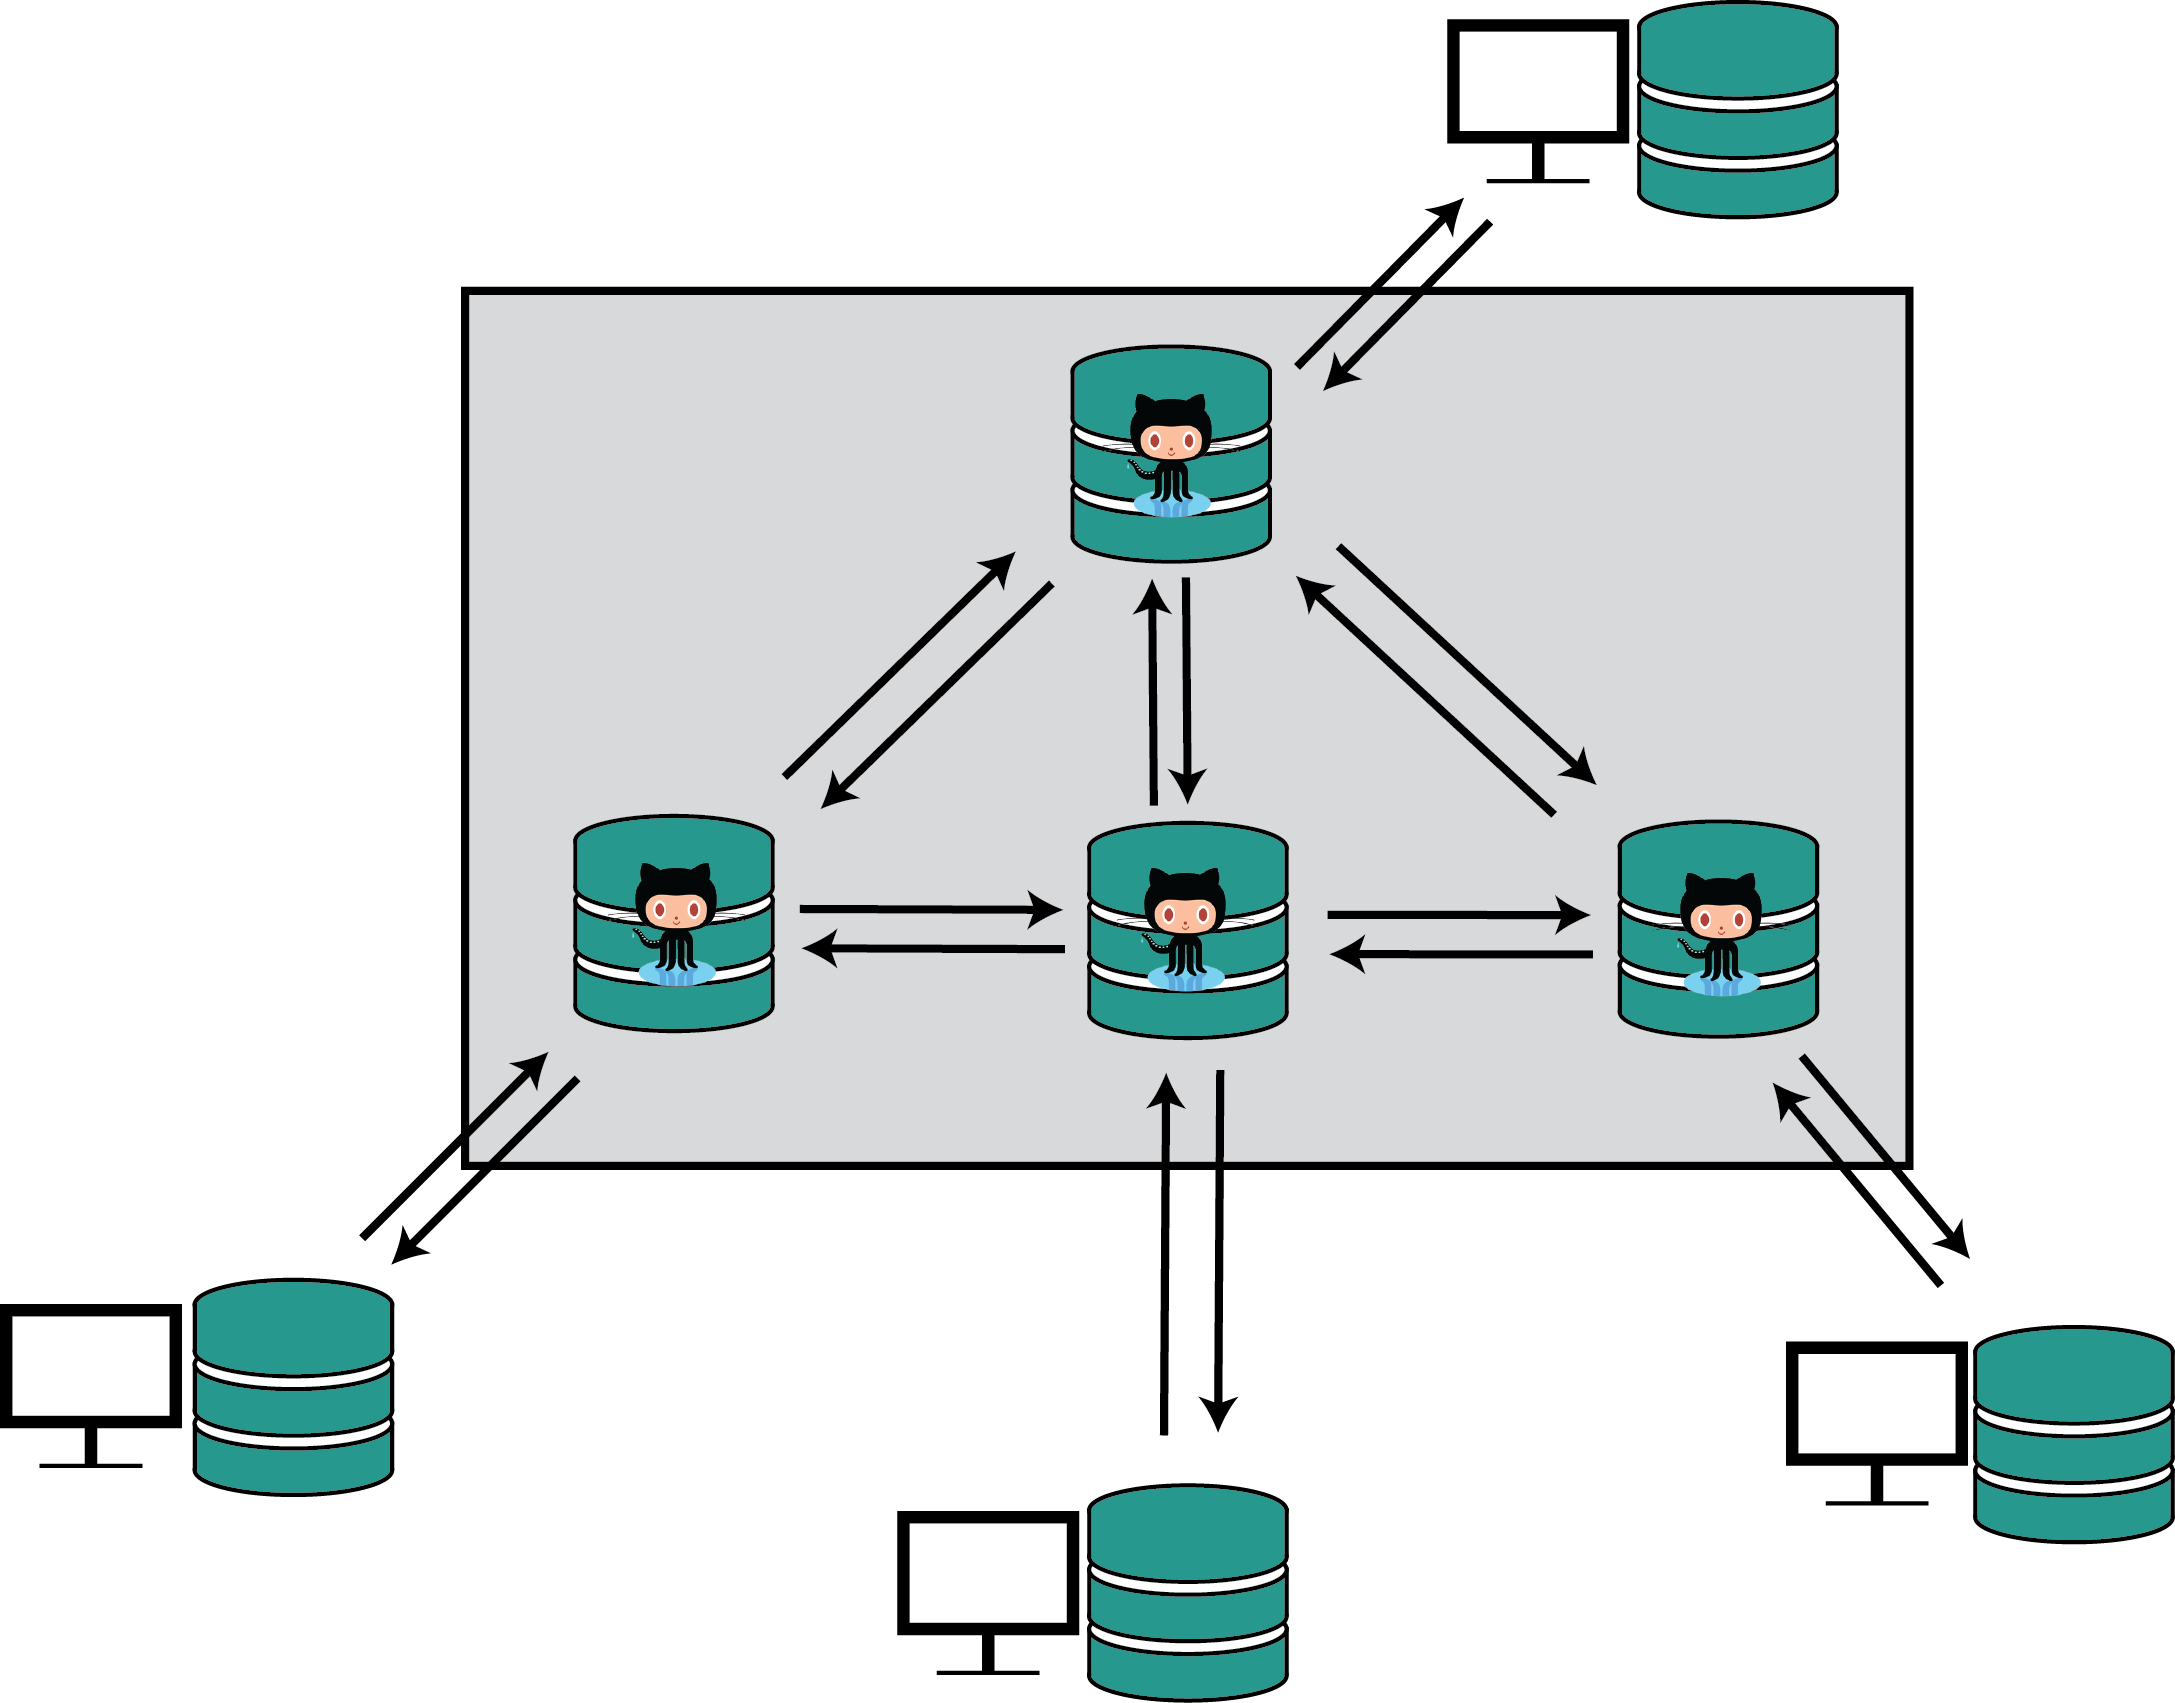
\includegraphics{../imgs/git_picture.png}}
\end{center}
\end{frame}

\begin{frame}
\frametitle{What we want version control with \texttt{Git} to look like:}
\begin{center}
\scalebox{0.45}{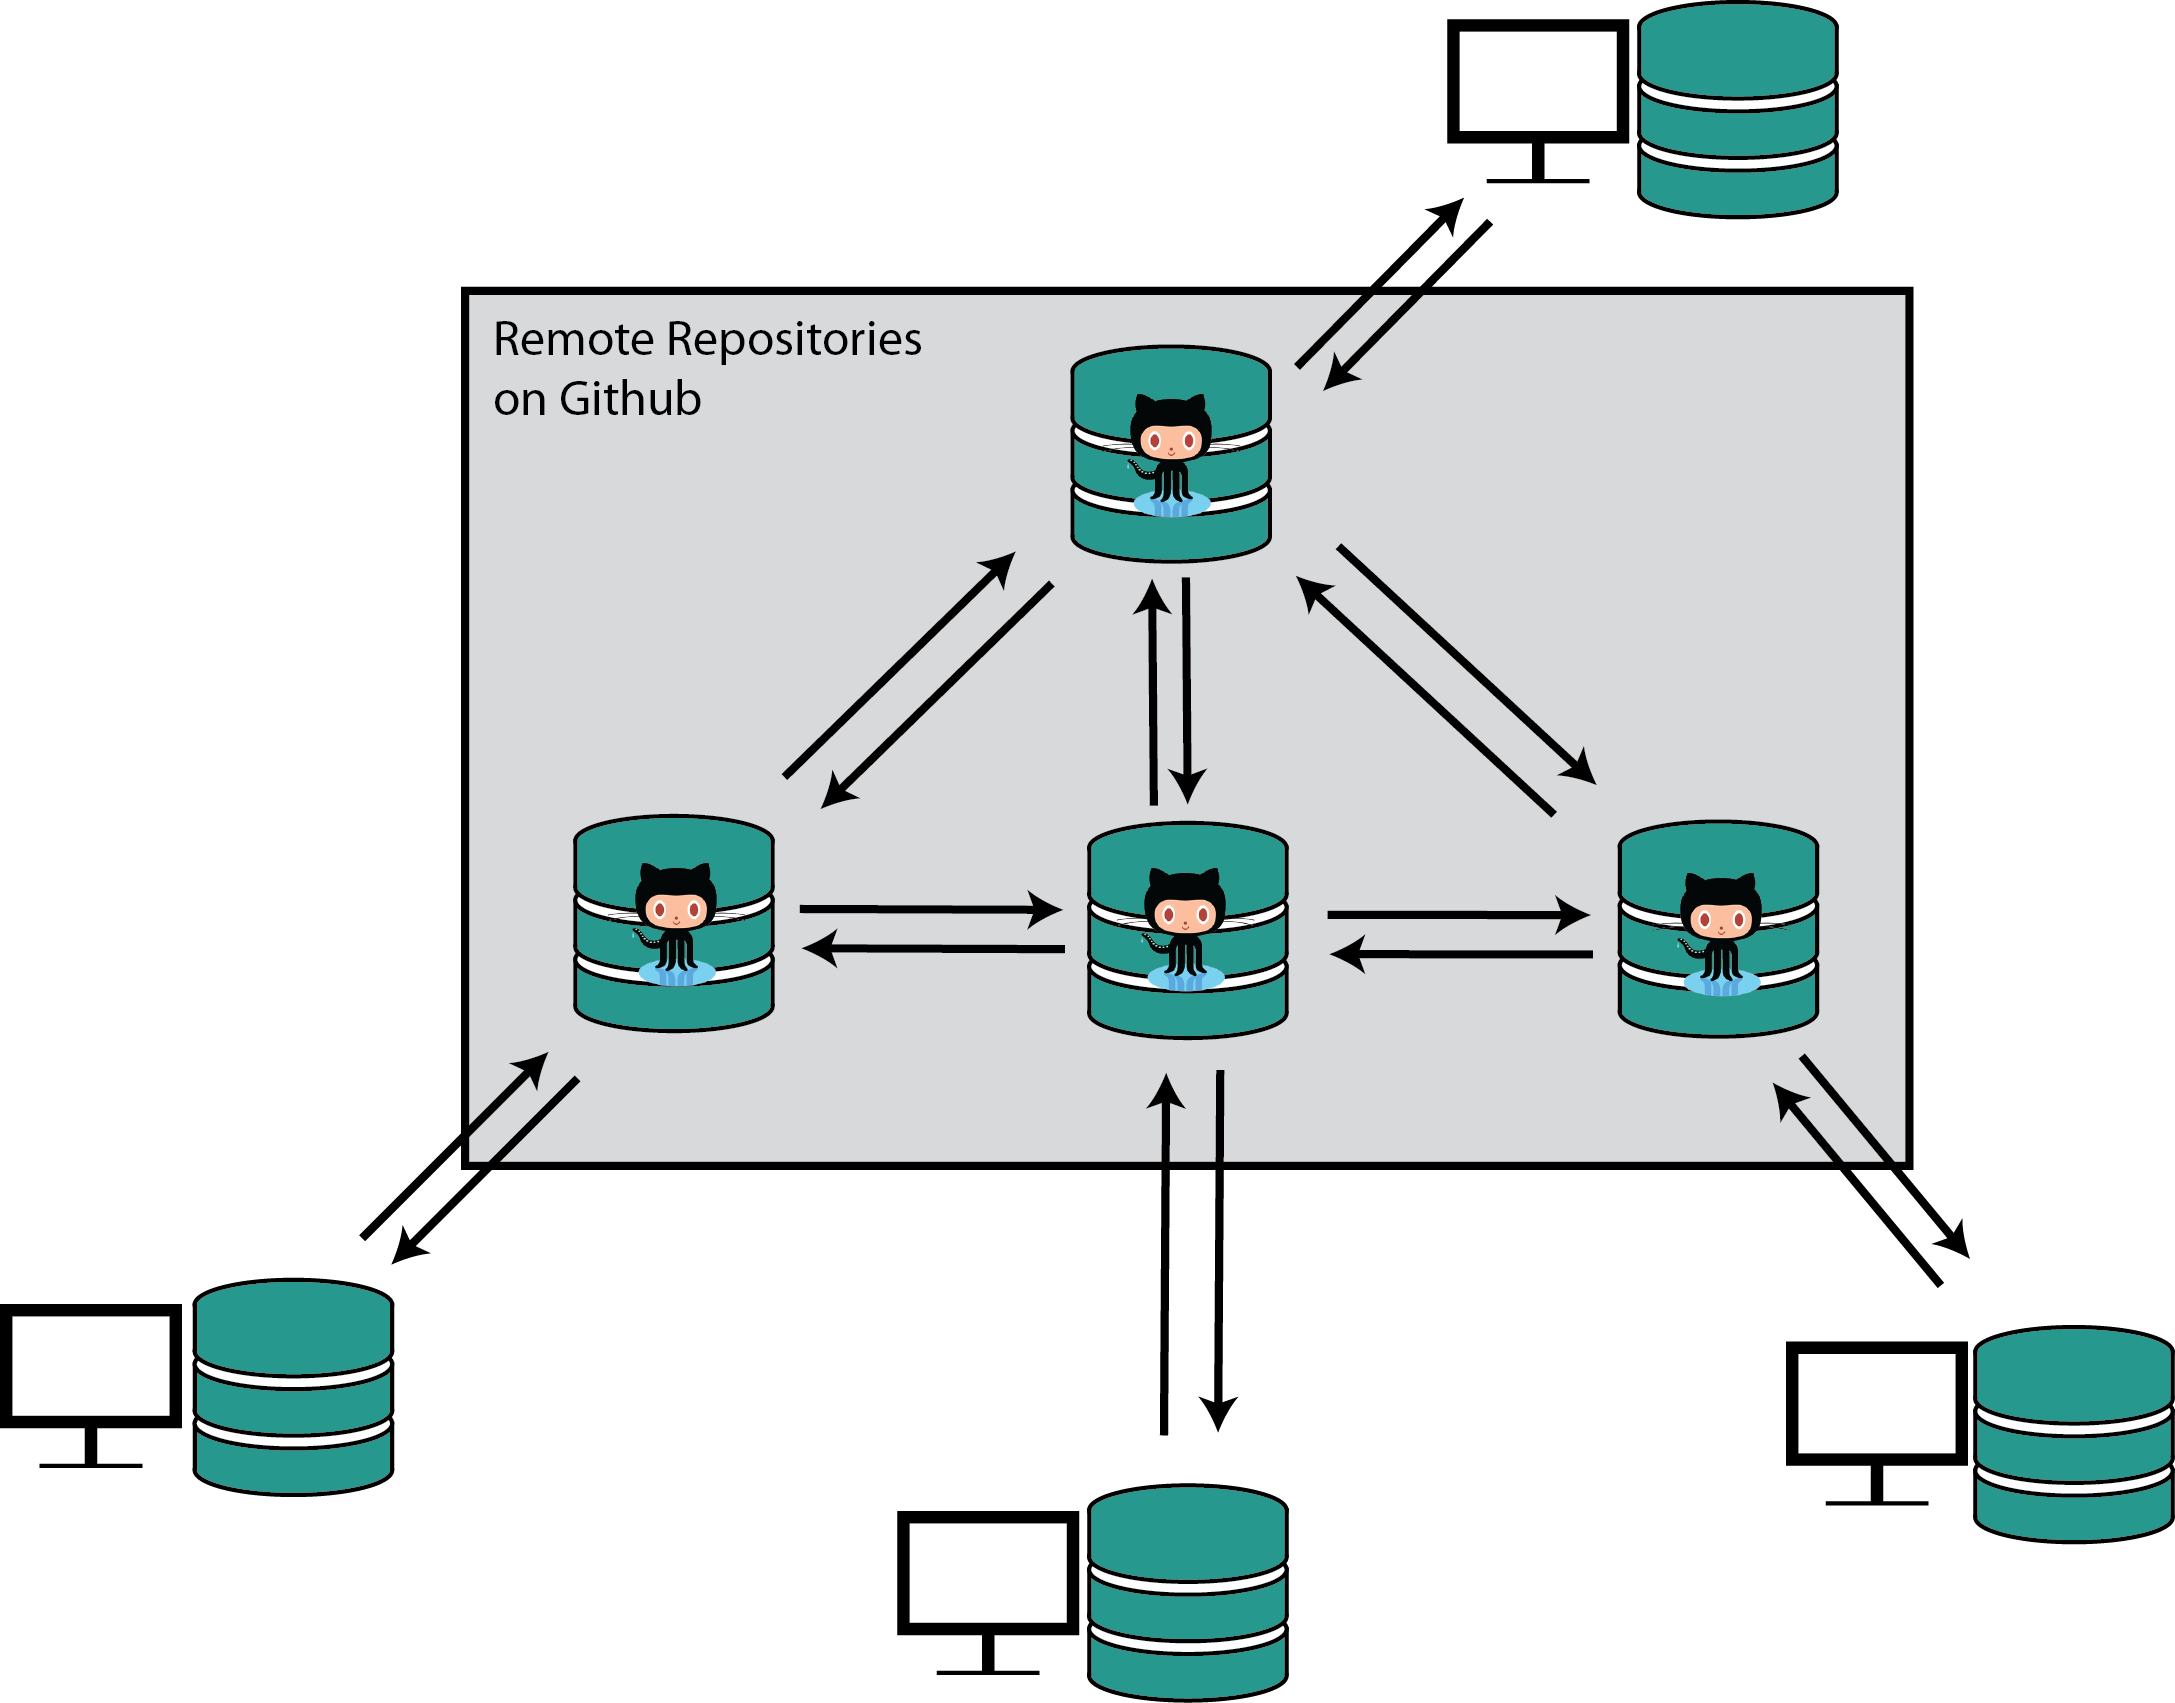
\includegraphics{../imgs/git_picture1.png}}

Github is a web hosting platform for Git projects. \pause

\textit{Let me show you Github.}
% Go to Github and show them how to make a new repository using my practice repository
% By default, git repositories hosted on github will be public - pay for private
% if you decide to create a README file, a Licence, or a .gitignore on github, it will automatically commit
% Use ssh protocols
\end{center}
\end{frame}

\begin{frame}[fragile]
\frametitle{Now that I have made a repository on Github, this is what I have:}
\begin{center}
\scalebox{0.7}{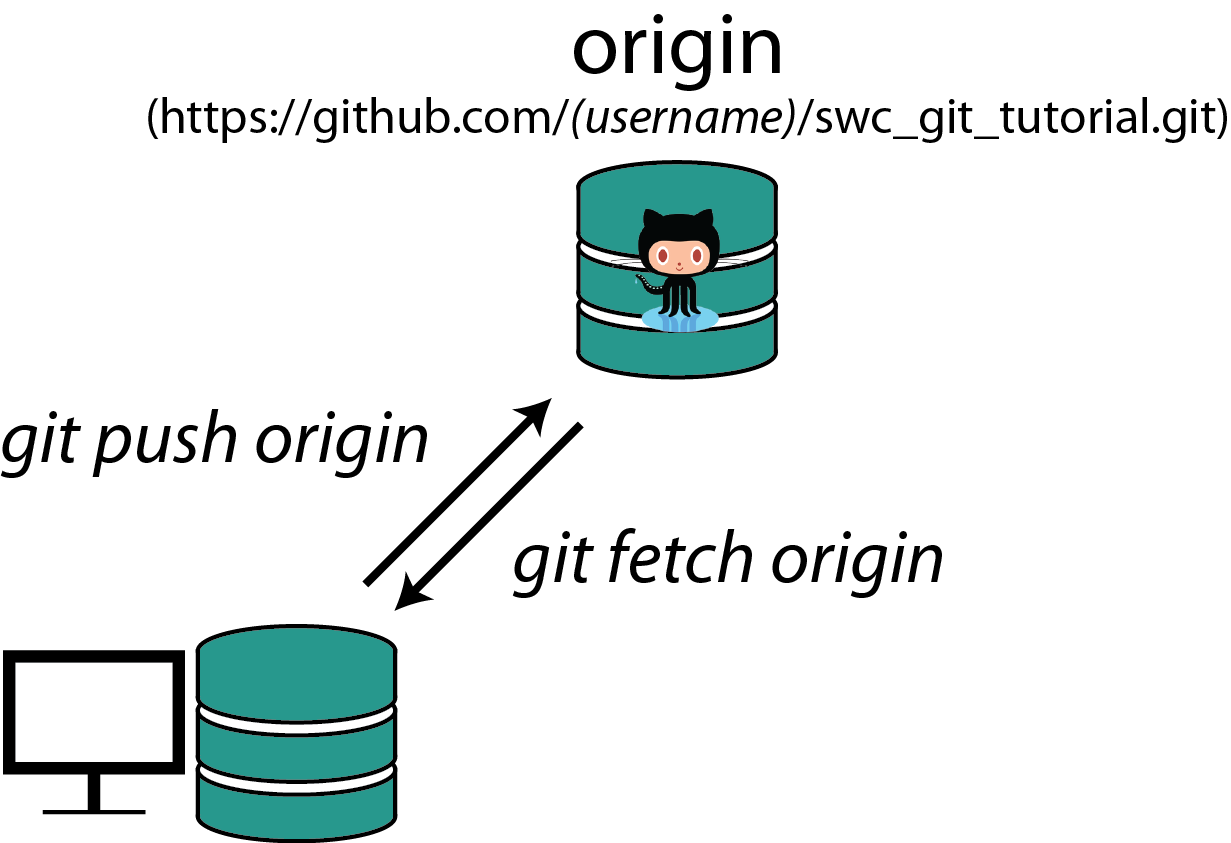
\includegraphics{../imgs/after_github.png}}\pause

\begin{verbatim}
                      git remote -v
\end{verbatim}
\end{center}
\end{frame}

\begin{frame}
\frametitle{Working with a collaborator}
\begin{center}
\scalebox{0.5}{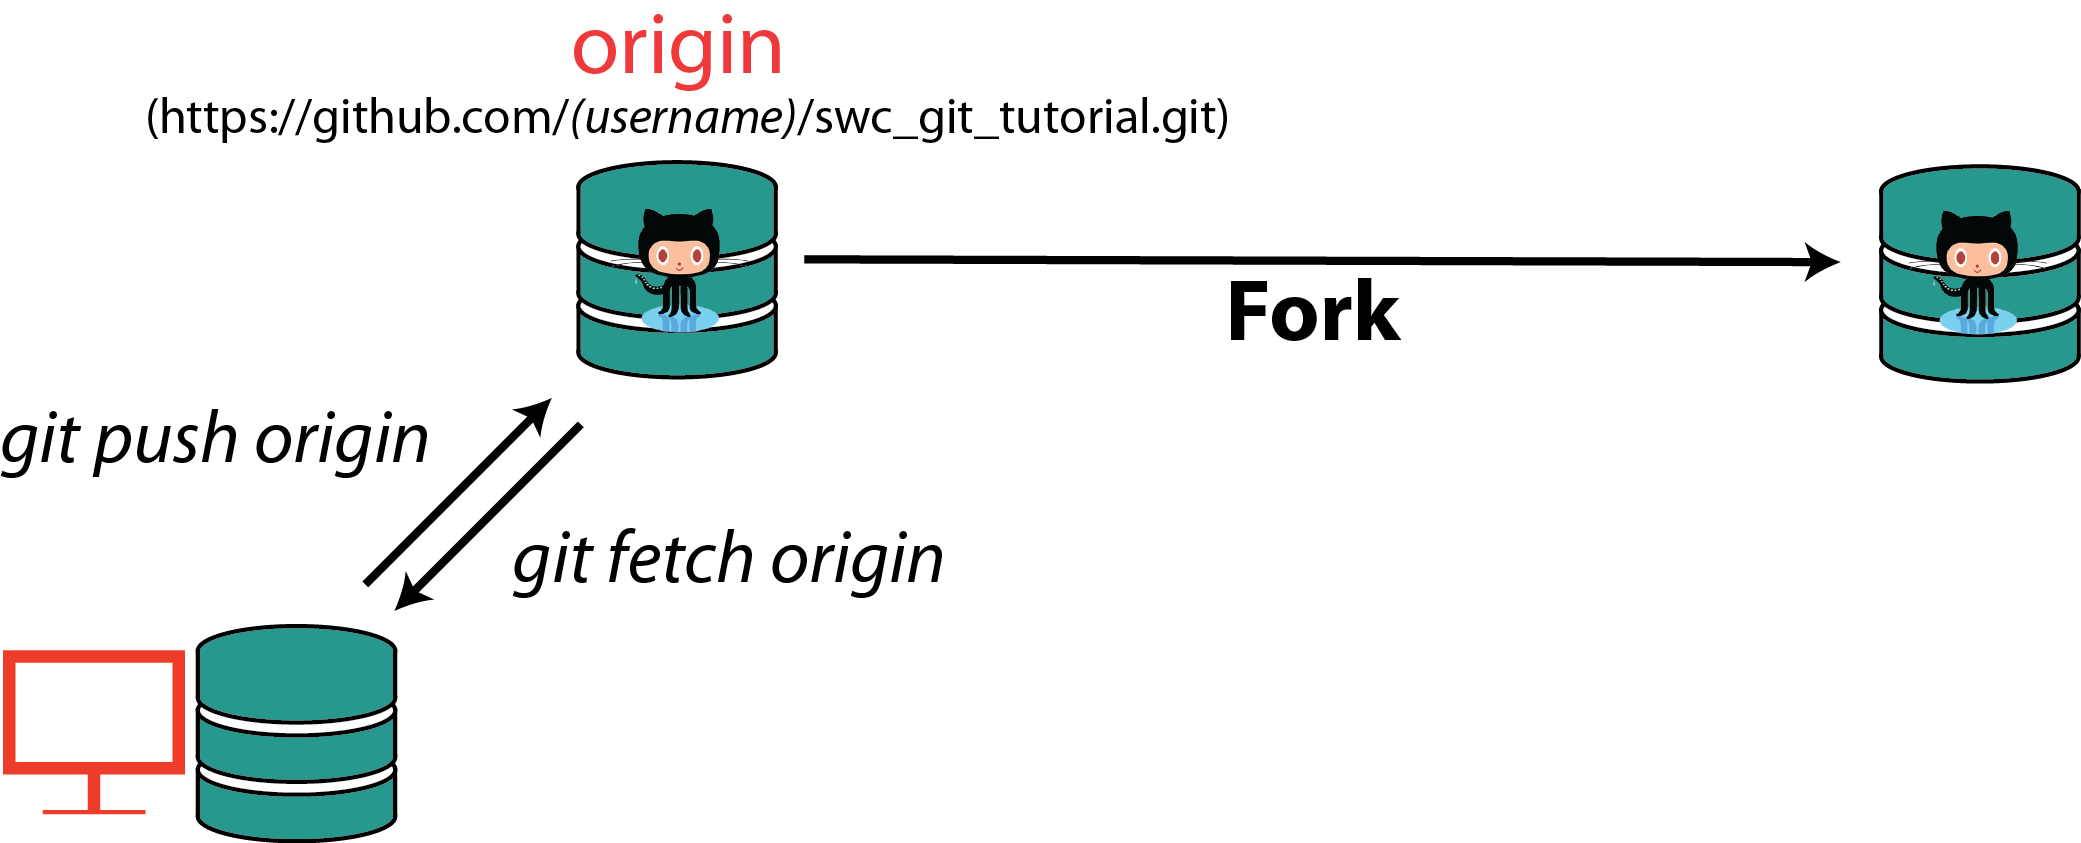
\includegraphics{../imgs/fork.png}}
\end{center}
\end{frame}


\begin{frame}
\frametitle{Working with a collaborator}
\begin{center}
\scalebox{0.5}{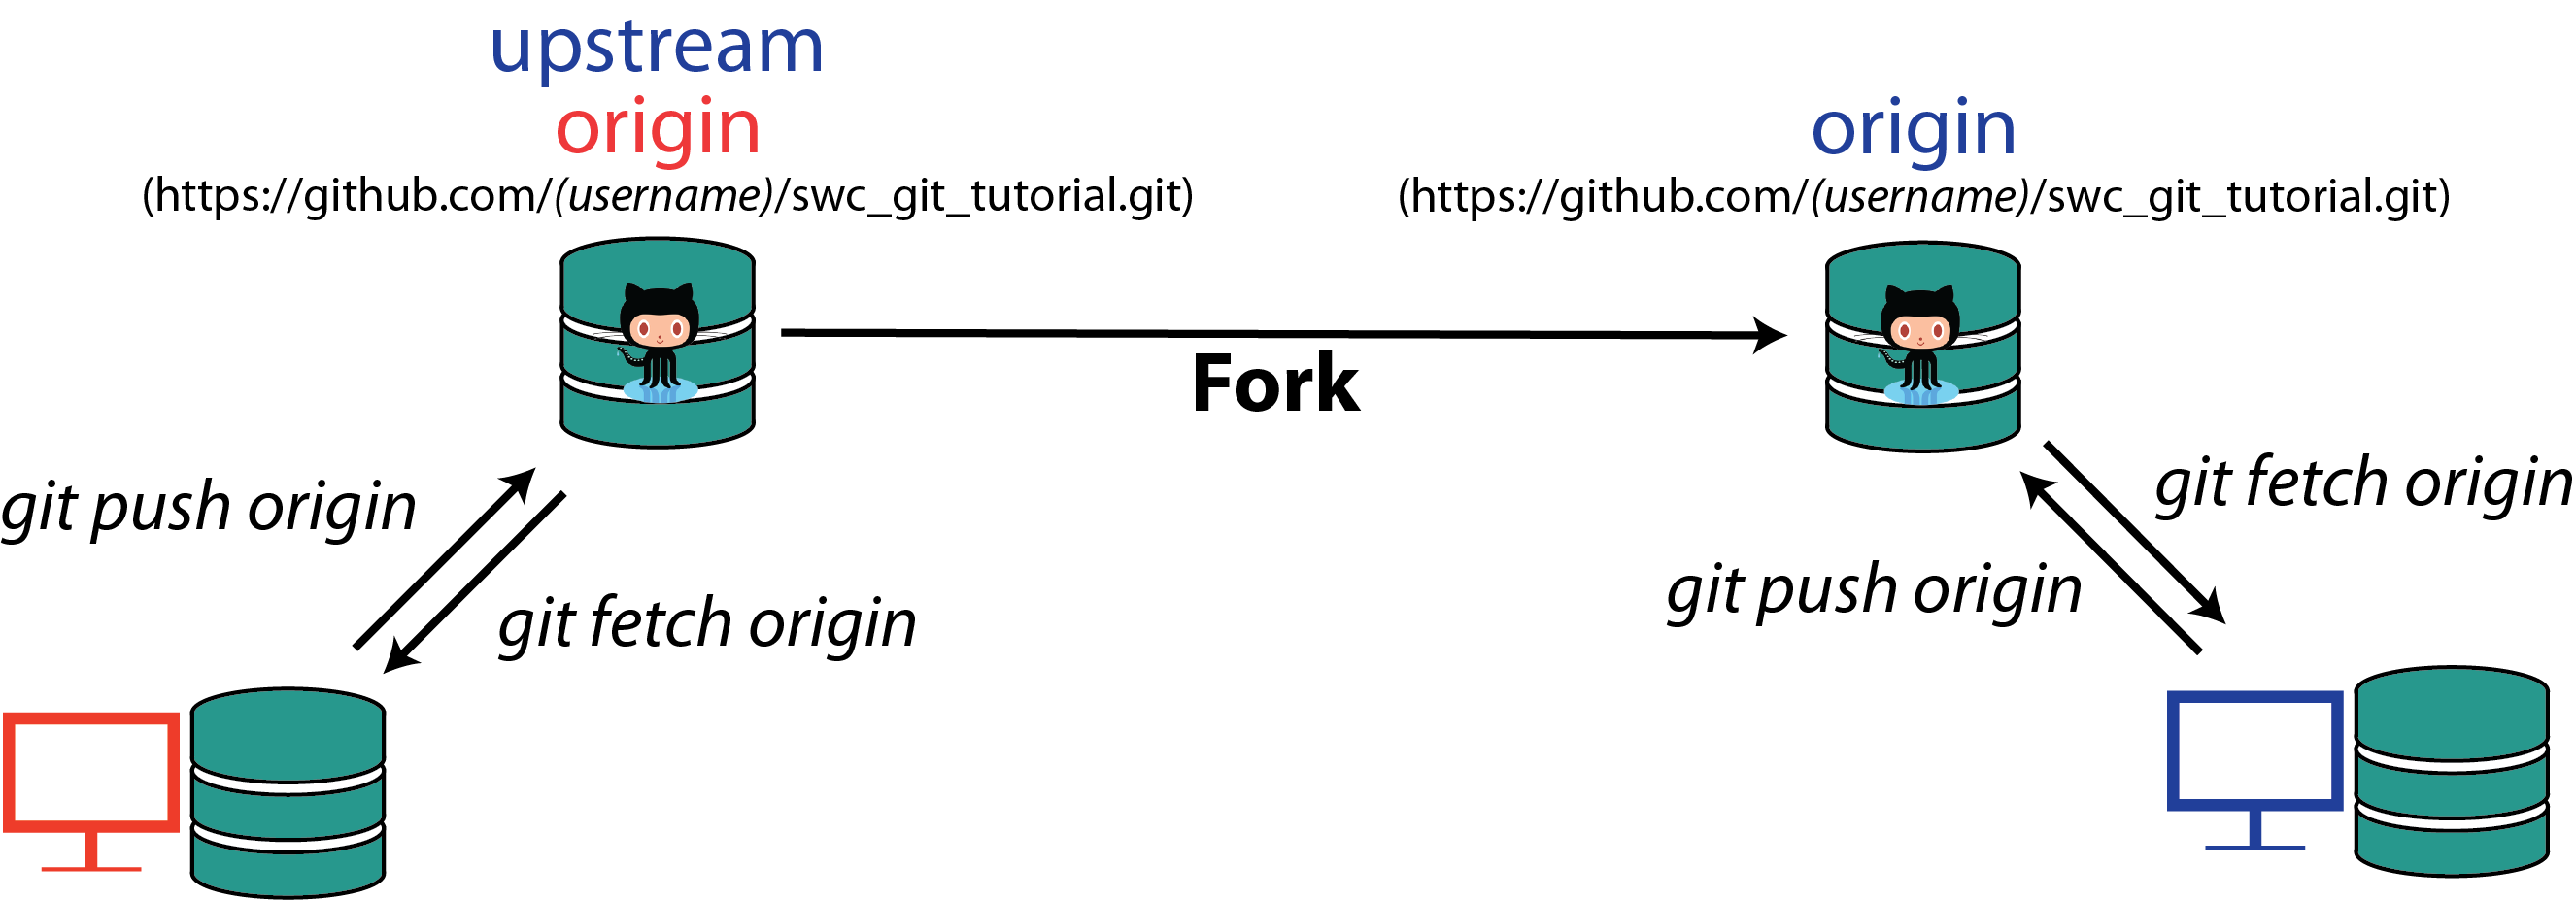
\includegraphics{../imgs/fork1.png}}
\end{center}
\end{frame}

\begin{frame}
\frametitle{Working with a collaborator}
\begin{center}
\scalebox{0.5}{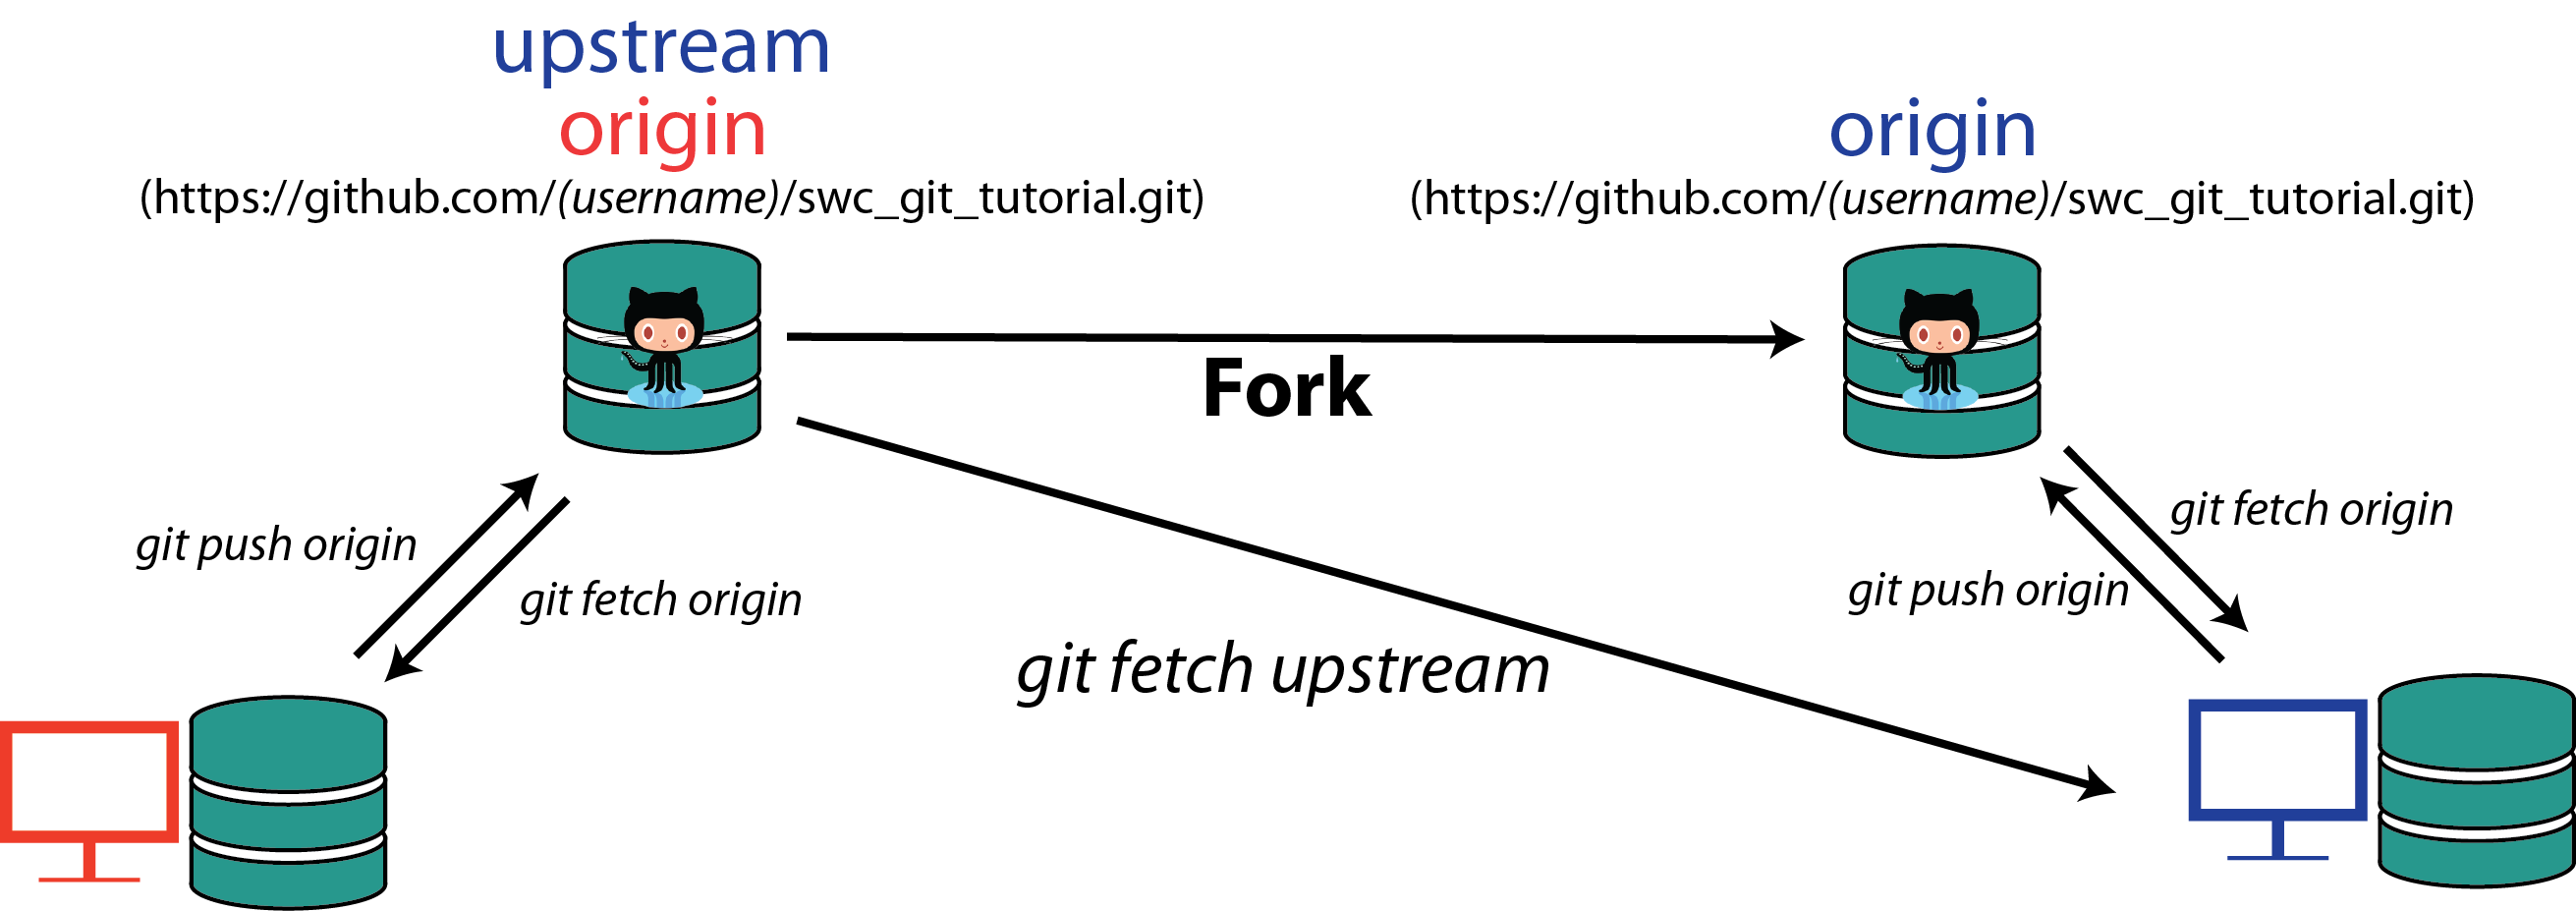
\includegraphics{../imgs/fork2.png}}
\end{center}
\end{frame}

\begin{frame}
\frametitle{Working with a collaborator}
\begin{center}
\scalebox{0.5}{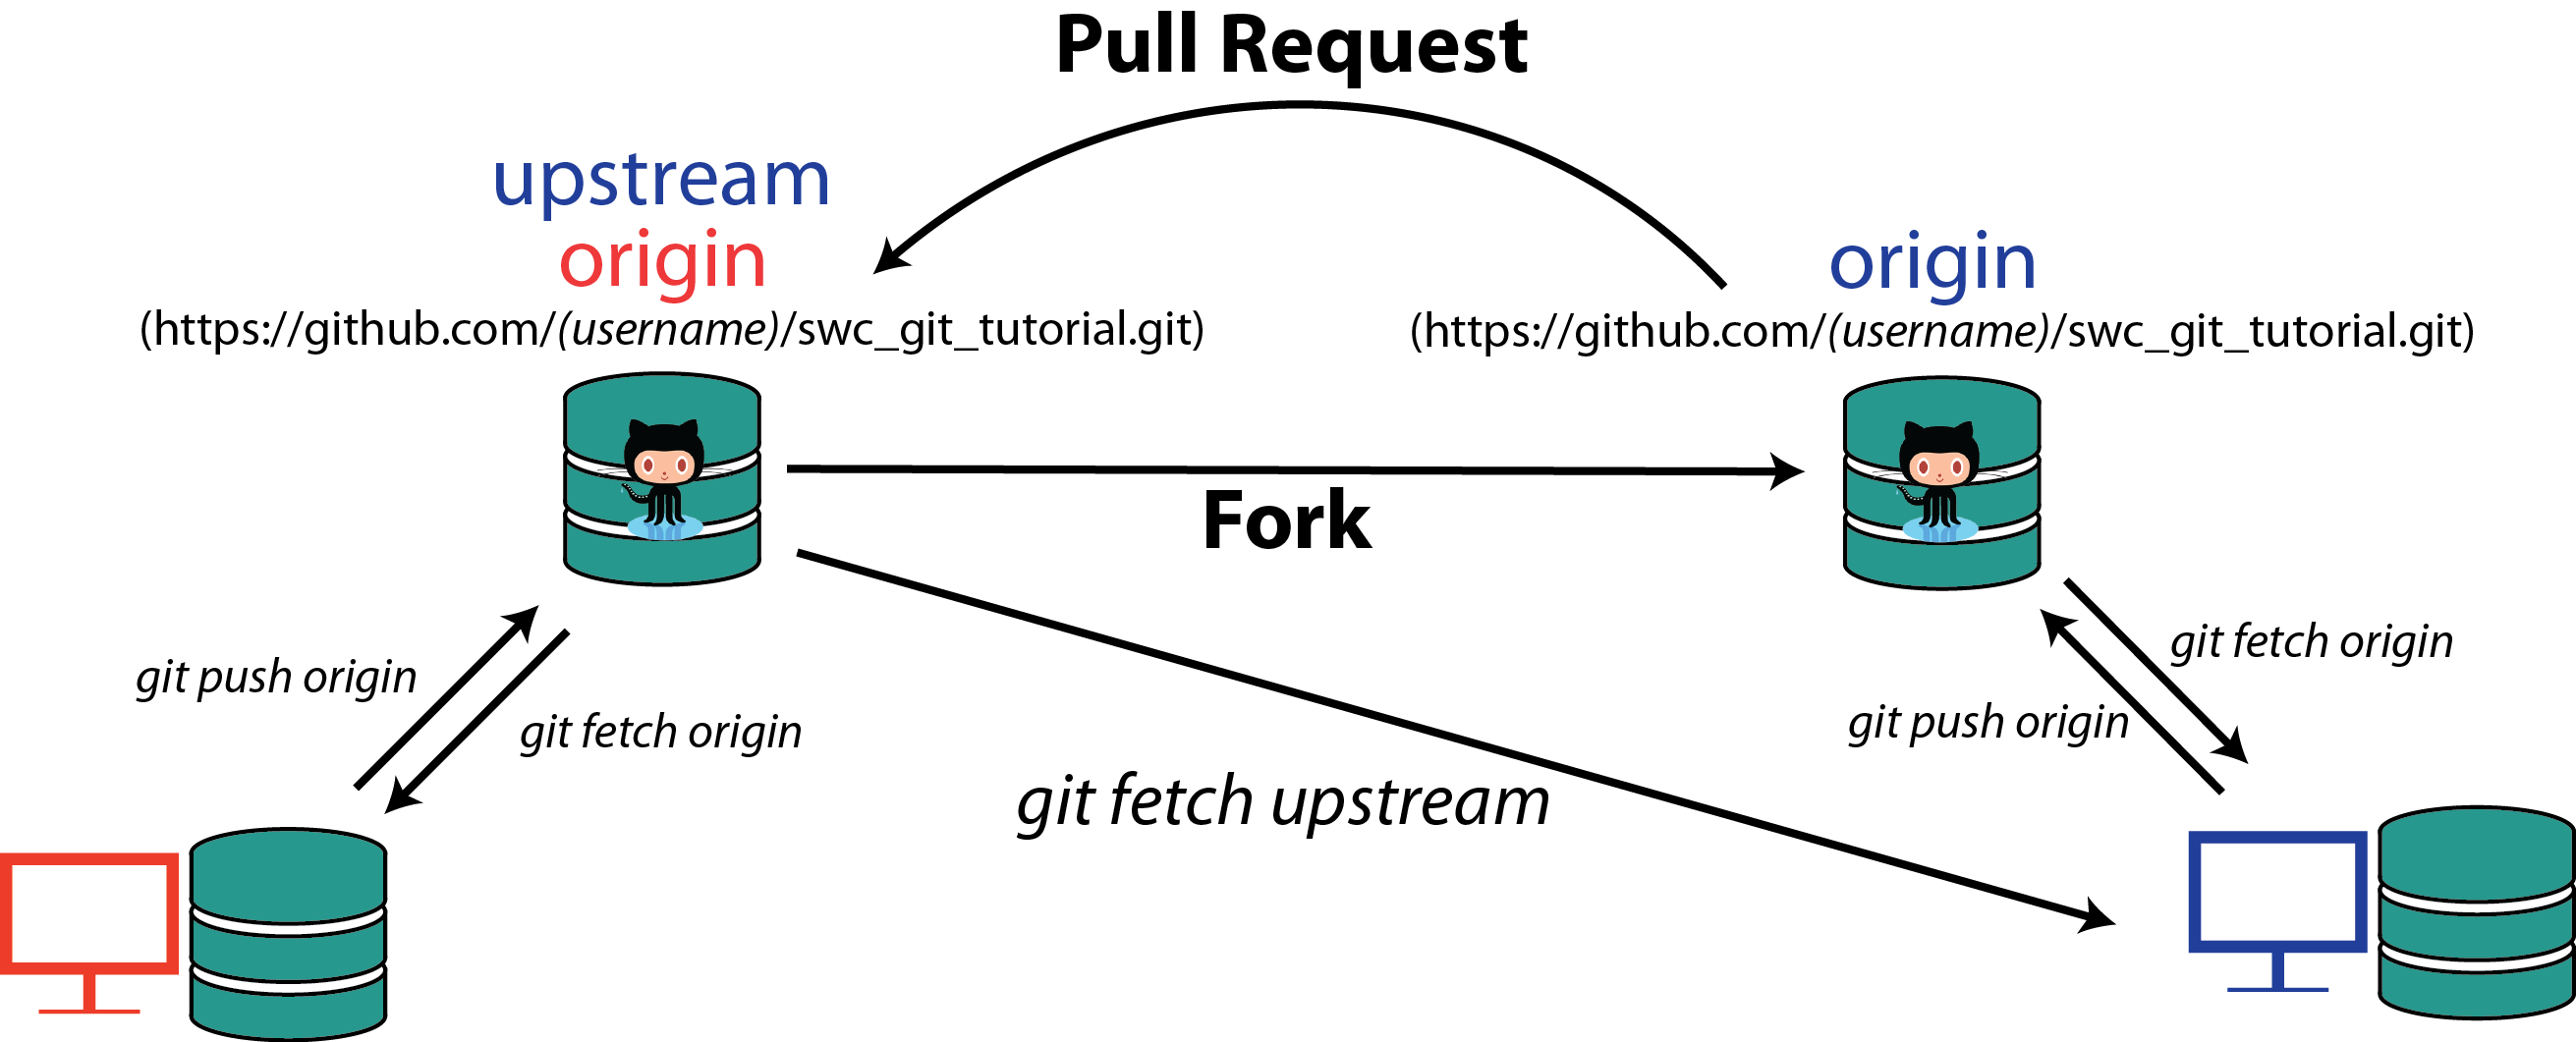
\includegraphics{../imgs/fork3.png}}
\end{center}
\end{frame}

\begin{frame}
\frametitle{Working with a collaborator (or two)}
\begin{center}
\scalebox{0.5}{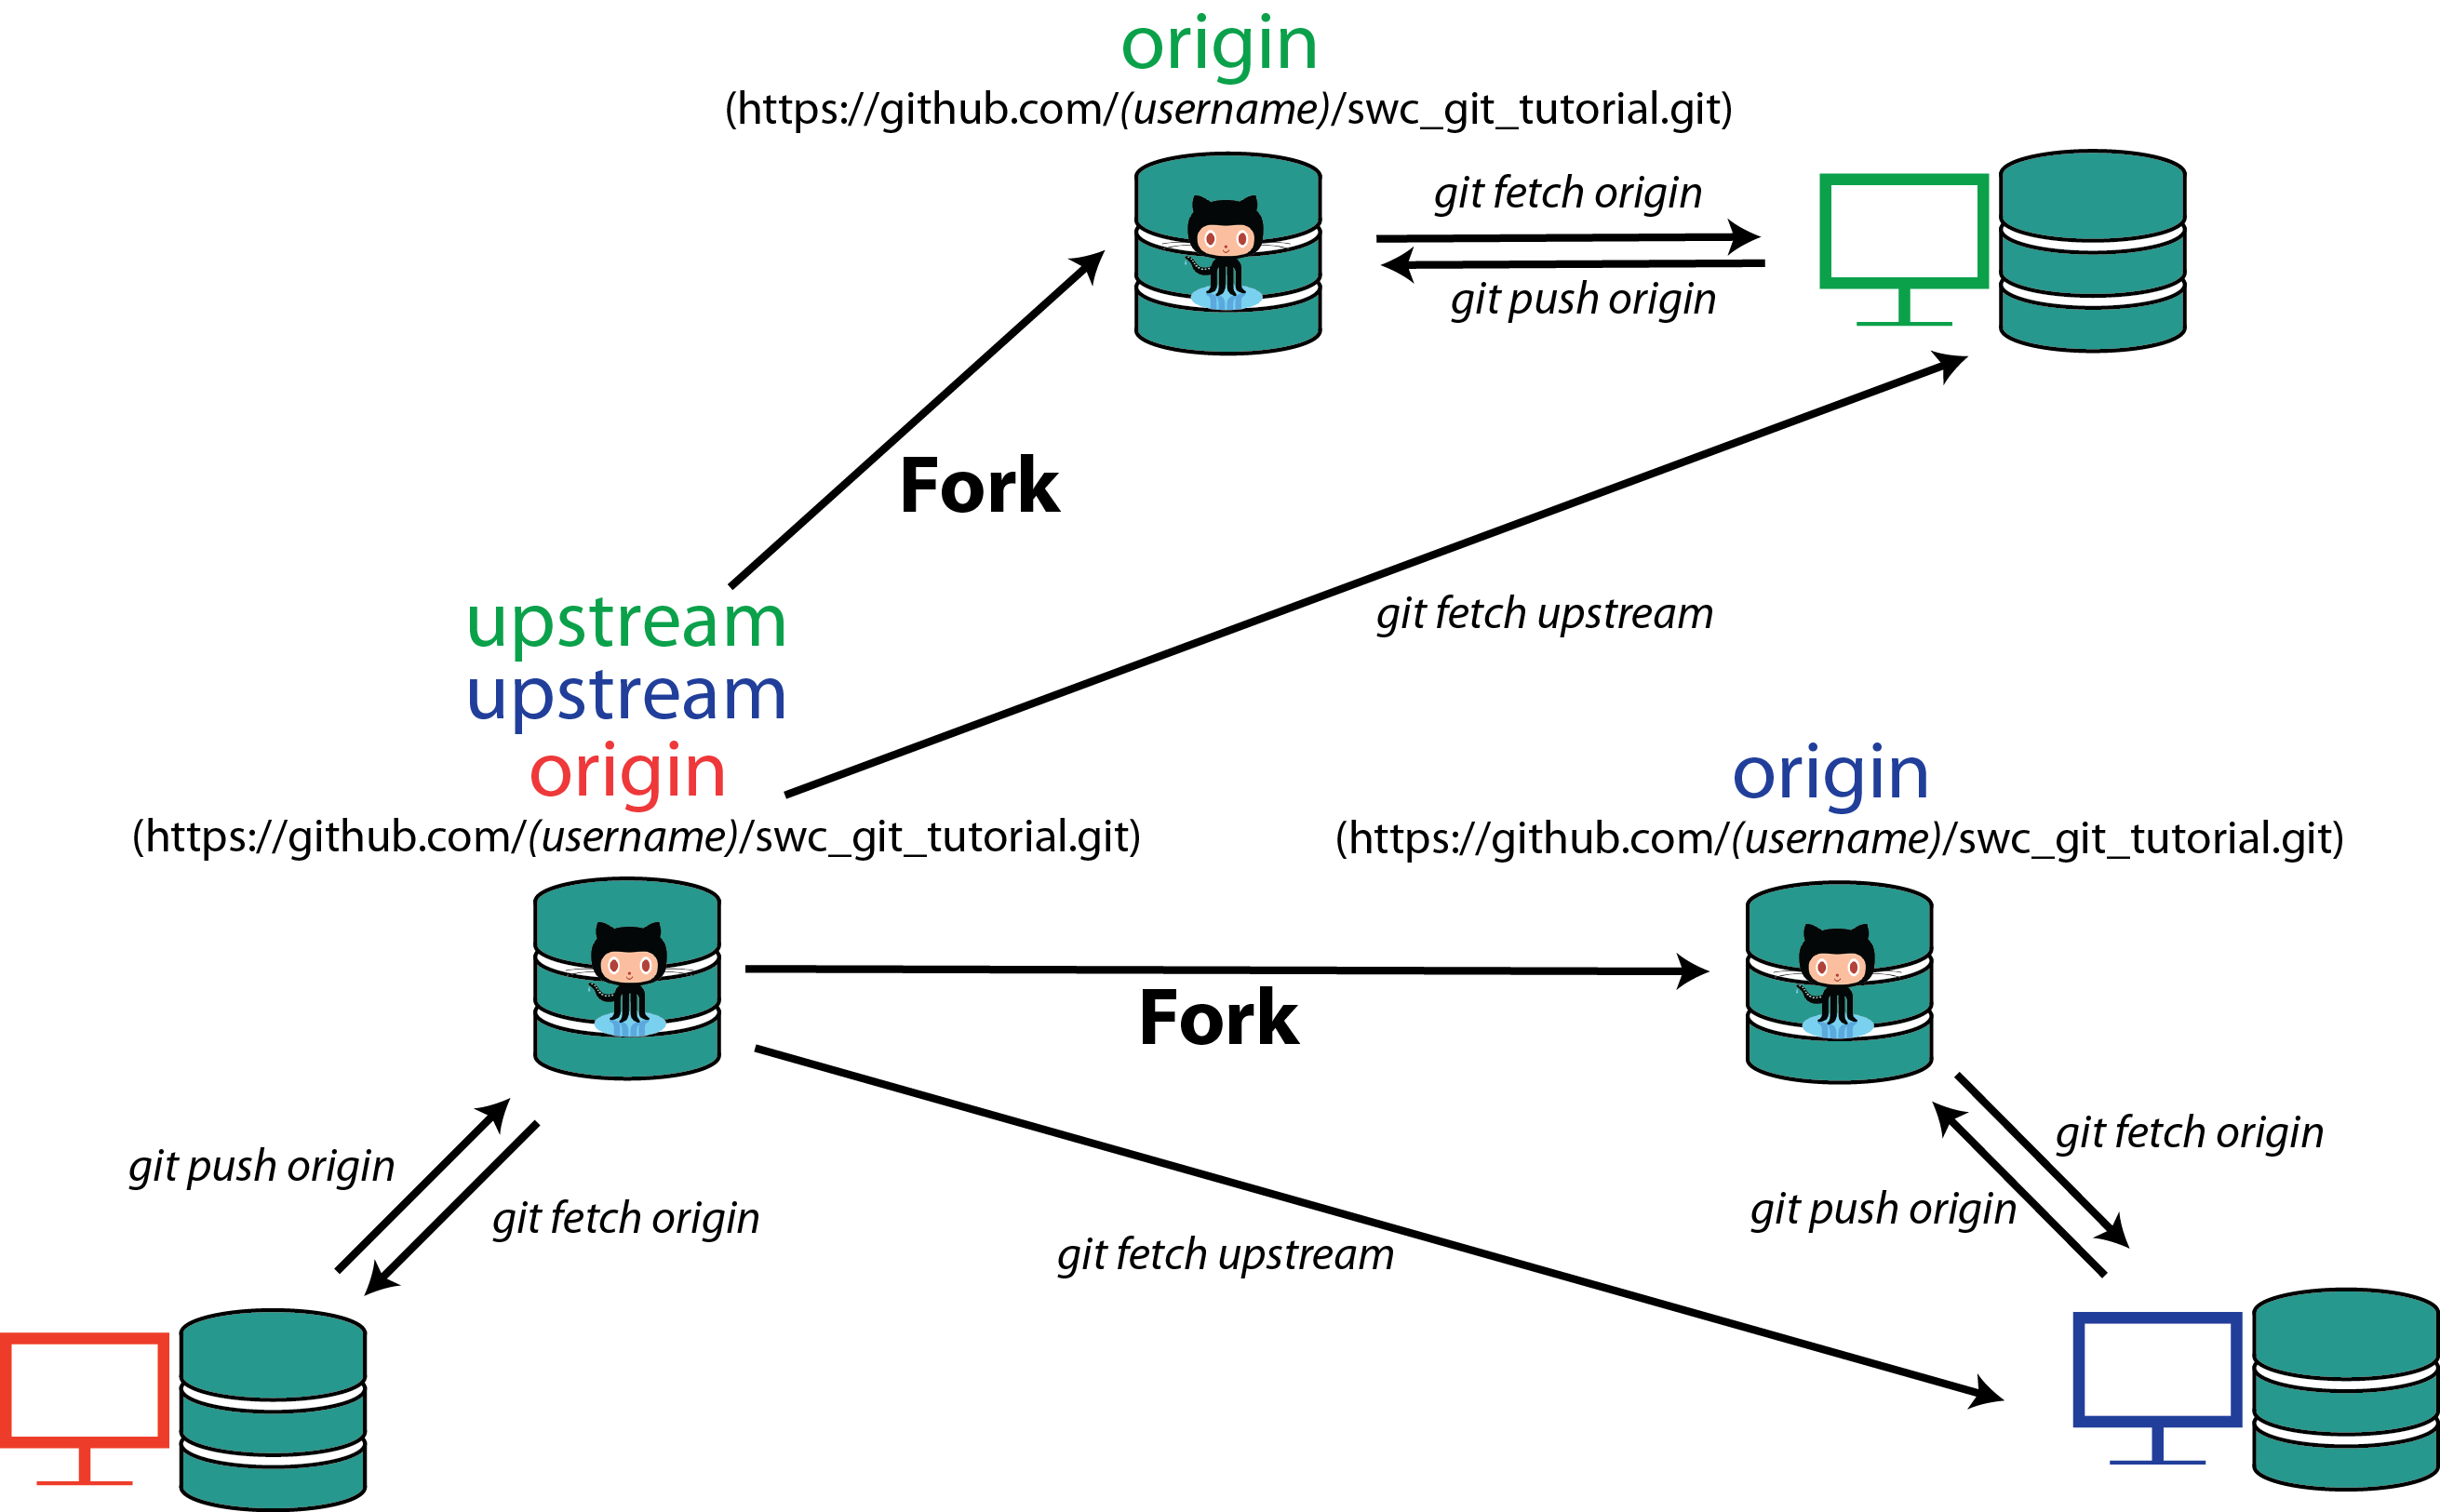
\includegraphics{../imgs/fork4.png}}
\end{center}
\end{frame}

\begin{frame}
\frametitle{Your Turn}
\begin{center}
Questions? \pause
\vspace{30pt}

You Try (30 mins)\\
\textbf{\textcolor{red}{Exercise 4}}
\end{center}
\end{frame}

\end{document}


